
\newcommand{\FigOverview}{
\begin{figure}[ht]
    \centering
    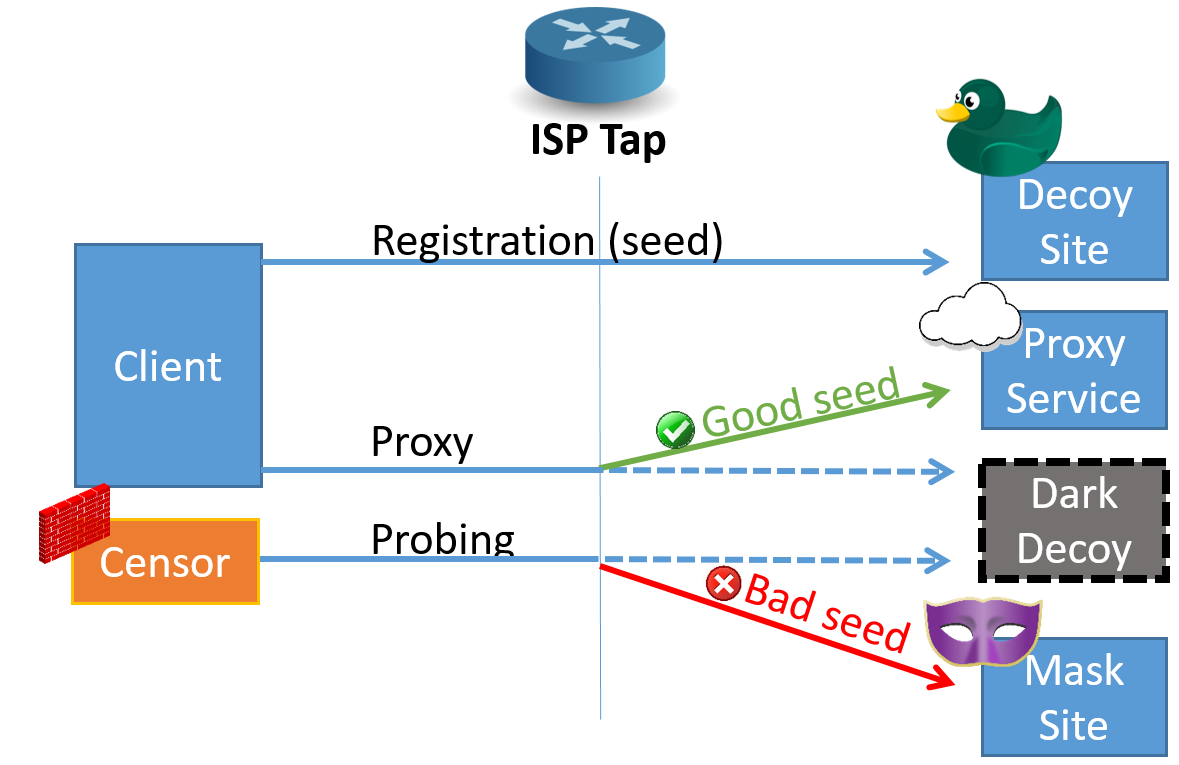
\includegraphics[width=0.9\linewidth,clip]{figures/dark-decoy-overview.png}
    \caption{\textbf{Dark Decoy Overview}\,---\, %
    }
    \label{fig:overview}
\end{figure}
}

\newcommand{\FigHighLevel}{
\begin{figure}[t]
    \centering
    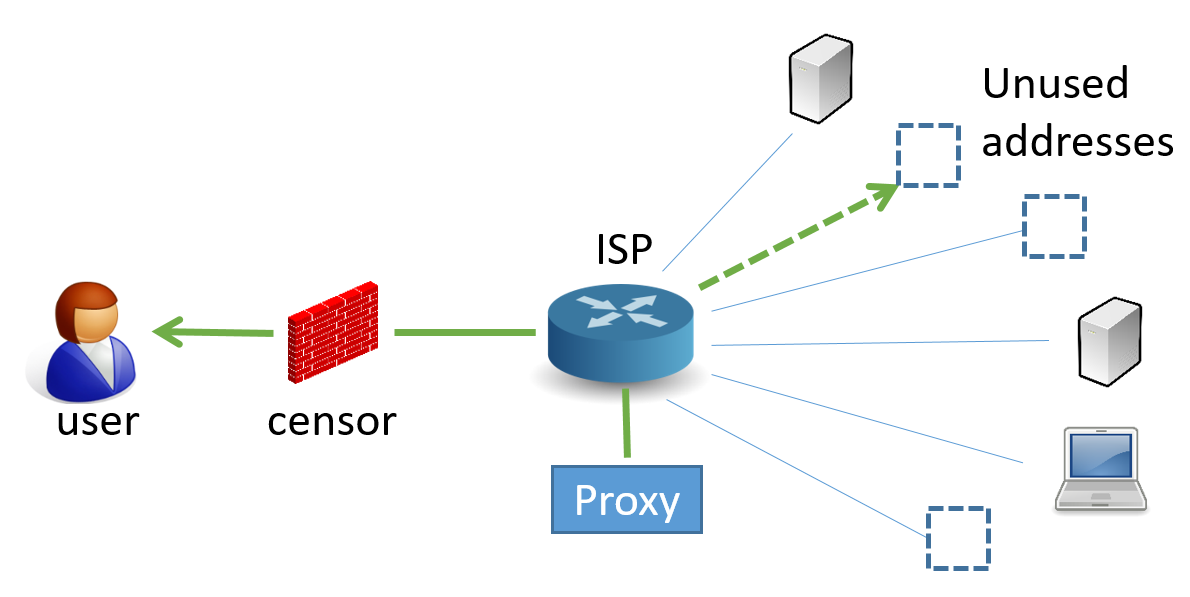
\includegraphics[width=0.9\linewidth,clip]{figures/high-level.png}
    \caption{\textbf{Dark Decoys}\,---\, %
    After registration, clients connect to unused (``dark'') addresses that pass
        by a cooperating ISP proxy station. The station communicates with the client
        as if it were the host at that address. To the censor, this
        connection appears to be with a legitimate one to a real host,
        making it difficult to distinguish from real hosts and block.
    }
    \label{fig:overview}
\end{figure}
}


\newcommand{\yes}{\CIRCLE}
\newcommand{\no}{\Circle}
\newcommand{\maybe}{\LEFTcircle}

\newcommand{\TabCompare}{
\begin{table*}[ht]
    \centering
    \begin{tabular}{l|cccccccc}
            % Multiflow? Waterfall?
            & \rot{Telex~\cite{telex}} &
            \rot{Cirripede~\cite{cirripede}} &
            \rot{Decoy Routing~\cite{curveball}} &
            \rot{TapDance~\cite{tapdance}} & \rot{Rebound~\cite{rebound}} & \rot{Slitheen~\cite{slitheen}} & \rot{Waterfall~\cite{waterfall}} & \rot{\textbf{Dark Decoys}} \\
            \hline
                                      %Telex Cirr  DR     TD      RB    Slth   Water  DD
            No inline blocking        & \no & \no  & \no & \yes  & \no  & \no  & \no  & \yes \\
            Handles asym. routing     & \no & \yes & \no  & \yes & \yes & \no  & \yes & \yes \\
            Currently deployed        & \no & \no  & \no  & \yes & \no  & \no  & \no  & \no \\
            Replay attack resistant   &\yes & \yes & \yes & \no  & \yes & \yes & \yes & \yes \\
            Traffic analysis resitant &\no  & \no  & \no  & \no  &\maybe& \yes &\maybe& \no \\
            Uses unused addresses     & \no & \no  & \no  & \no  & \no  & \no  & \no  & \yes \\
    \end{tabular}
    %\caption{\textbf{Refraction Networking schemes}\,---\,}
    \label{tab:compare}
\end{table*}
}



\newcommand{\FigImplementation}{
\begin{figure}[ht]
    \centering
    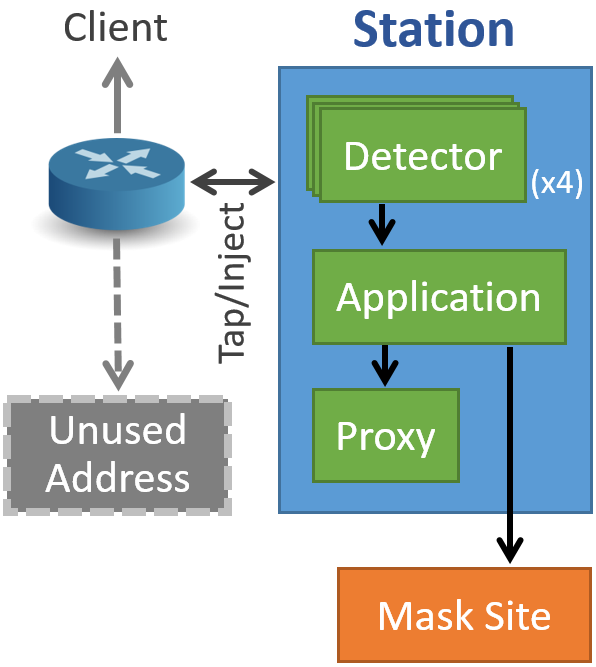
\includegraphics[width=0.7\linewidth,clip]{figures/implementation.png}
    \caption{\textbf{Station Architecture}\,---\, %
    }
    \label{fig:implementation}
\end{figure}
}


